\documentclass[11pt]{article}
\usepackage{amsmath, amssymb}
\usepackage[margin=1in]{geometry}
\usepackage{enumitem}
\usepackage{graphicx}
\usepackage{float}
\usepackage{caption}
\usepackage{booktabs}
\usepackage{hyperref}
\graphicspath{{figures/}}
\captionsetup{font=small}

\title{Strictly greedy $O(N^2)$ ground states for Stefan's Fig.~6 QUBO ensemble}
\author{}
\date{2026-11-18}

\begin{document}
\maketitle

\section*{Setup:}

\noindent\textbf{Problem:} Minimize
\[
  E(x) = -\sum_{i,j} q_{ij}\, x_i x_j, \qquad x_i \in \{0,1\},\ i = 1,\dots,N,
\]
where the sum runs over both orders of each pair. The matrix $q$ is symmetric with zero diagonal; each off-diagonal
entry is nonzero with probability 0.1 and then an integer drawn uniformly from $[-100, 100]$. The quantity reported is the
energy density $e = E/N^{3/2}$, averaged over random instances, for $N = 31$ to $4095$.

\noindent\textbf{Stefan's Fig.~6 table:} For each $N$, the average of $e$ over 600 to 100\,000 instances, with its
standard error, obtained with Stefan's own heuristic (his words). It is the only reference we score against. The
error of a method at a given $N$ is $(\langle e\rangle - e_{\rm table})/|e_{\rm table}|$; negative means lower
(better) energies than the table.

\noindent\textbf{Spin form:} With $s_i = 2x_i - 1 \in \{-1,+1\}$,
\[
  E = \tfrac12 H - \tfrac14 \sum_{i,j} q_{ij}, \qquad
  H = -\sum_{i<j} q_{ij}\, s_i s_j - \sum_i h_i s_i, \qquad h_i = \sum_j q_{ij},
\]
so the QUBO is a spin glass in which every spin also feels the row sum $h_i$ of $q$ (the field bias). The local field
on spin $i$ is
\[
  f_i = h_i + \sum_{j} q_{ij}\, s_j ,
\]
where, during the greedy pass, spins not yet fixed have $s_j = 0$. Once every spin is fixed, flipping spin $i$ changes
the energy by
\[
  \Delta E_i = s_i f_i ,
\]
so the best sign of a spin is $s_i = \operatorname{sign}(f_i)$, and a flip lowers $E$ only if $s_i f_i < 0$.
Fixing or flipping one spin updates every $f_j$ by $\pm q_{jb}$: one row of $q$, $O(N)$ work.

\noindent\textbf{Strictly greedy:} Every spin is fixed exactly once, along its current local field, and is never
undone. Afterwards the only moves allowed are single flips that strictly lower $E$. No trial-and-undo, restarts or
copies of the state. The only freedom is the \emph{order} in which spins are fixed, and the total work must stay
$O(N^2)$.

\section*{Algorithms:}

All three start from $s = 0$, $f = h$, and end with the same descent.

\noindent\textbf{Original greedy (baseline):} Repeat $N$ times: fix the unfixed spin with the largest $|f_b|$ to
$s_b = \operatorname{sign}(f_b)$ and update $f$.

\noindent\textbf{Confidence greedy:} Keep, for every spin, the remaining coupling strength
\[
  R_i = \sum_{j\ \text{unfixed}} q_{ij}^2 ,
\]
which measures how much $f_i$ can still change: the part of $f_i$ still to come is a sum of $\pm q_{ij}$ terms of
typical size $\sqrt{R_i}$. Repeat $N$ times: fix the unfixed spin with the highest confidence
\[
  \text{score}_i = \frac{f_i^2}{(R_i + c)^{5/4}}, \qquad c = 0.01\,\overline{R} + 1,
\]
to $s_b = \operatorname{sign}(f_b)$, then update $f_j \mathrel{+}= q_{jb} s_b$ and $R_j \mathrel{-}= q_{jb}^2$.
A large field that can still change sign is fixed later than a smaller one that is already settled. The exponent $5/4$
and the regularizer $c$ ($\overline{R}$: mean of $R$ at the start) were tuned on random instances; $5/4$ works better
than $1$, which would be the squared signal-to-noise ratio $f_i^2/R_i$.

\noindent\textbf{Look-ahead greedy:} The same, plus a running guess $p_j \in \{-1,+1\}$ of the sign each unfixed spin
will take (start: $p_j = \operatorname{sign}(h_j)$), used only to choose the order. It gives the predicted rest of the
field and an anticipated field
\[
  \begin{gathered}
  P_i = \sum_{j\ \text{unfixed}} q_{ij}\, p_j, \qquad u_i = f_i + A_t P_i, \\
  A_t = A\left(0.6 + 2\,\frac{n_{\rm unfixed}}{N}\right), \qquad A = \min(0.4,\ 0.05\log_2 N - 0.12).
  \end{gathered}
\]
Each step fixes the spin with the highest
\[
  \text{score}_i =
  \begin{cases}
    u_i^2/(R_i+c)^{5/4} & \text{if } u_i f_i > 0,\\
    0.1\, f_i^2/(R_i+c)^{5/4} & \text{otherwise},
  \end{cases}
\]
still along its actual field, $s_b = \operatorname{sign}(f_b)$, so a spin whose actual and anticipated fields disagree is
held back. Then it corrects one guess: among unfixed spins with $u_m p_m < 0$, the one with the largest $|u_m|$ gets
$p_m \to -p_m$, and $P$ is updated (one more row).

\noindent\textbf{Descent (all three):} Repeatedly flip the spin with the most negative $s_i f_i$ until no flip lowers
$E$. It makes only about $0.01N$ flips.

\noindent\textbf{Cost:} Each fixing step is one $O(N)$ scan plus one (look-ahead: at most two) $O(N)$ row updates,
so the total is about $2N^2$ ($3N^2$) operations: $O(N^2)$.

\section*{Summary:}
\begin{itemize}[nosep]
  \item \textbf{Two strictly greedy algorithms at $O(N^2)$ cost:} Running time grows as $N^2$ for all three variants.
  On one Apple-silicon core at $N = 1023$: 1.1\,ms (original), 2.0\,ms (confidence), 3.2\,ms (look-ahead); at
  $N=4095$: 17, 32 and 48\,ms (Fig.~\ref{fig:time}).
  \item \textbf{Both greedy rules land below the table:} Averaged over the 11 sizes, the confidence greedy is
  $0.60 \pm 0.04\%$ below the table and the look-ahead greedy $0.83 \pm 0.04\%$ below; the original greedy is above
  the table at small $N$ ($+0.56\%$ at $N=31$). At $N = 31$ both new rules agree with the table within error
  (Fig.~\ref{fig:energy}, Table~\ref{tab:err}).
  \item \textbf{The lead shrinks at the largest size:} At $N = 4095$ the margin drops to $-0.34\%$ (confidence) and
  $-0.65\%$ (look-ahead), from $-0.95\%$ and $-1.28\%$ at $N = 511$ (Fig.~\ref{fig:energy}).
  \item \textbf{The table follows $e_\infty + a/N$ closely:} Fitted for $N \ge 63$, $e = -10.805(3) + 30.4/N$ with
  $\chi^2/\nu = 1.1$, and the equation reproduces every table value from $N = 63$ to $4095$ within $\pm0.07\%$, inside
  the table's own error. An $N^{-2/3}$ correction fits much worse ($\chi^2/\nu = 23$). The same fit to the greedy data
  gives $e_\infty = -10.888(8)$ (confidence) and $-10.924(8)$ (look-ahead), but these are not reliable limits: the
  $N = 4095$ greedy points sit about $2\sigma$ above their lines (Figs.~\ref{fig:extrap}, \ref{fig:fitcheck}).
  \item \textbf{Why we land below the table:} The table is not exact ground states. Stefan describes it as the output of
  his heuristic, averaged over instances; each entry is an upper bound on the average ground-state energy. On the same
  instances as the greedy runs, a long tabu search (about 5000 times the greedy time at $N=1023$) finds energies that
  lie $0.9$ to $1.6\%$ below the table for $N \ge 63$, and agree with it at $N = 31$ ($+0.14 \pm 0.20\%$), where a
  heuristic almost surely finds the true ground states. Greedy sits between the two: $0.18$--$0.62\%$ (confidence)
  and $0.11$--$0.30\%$ (look-ahead) above the best found (Fig.~\ref{fig:best}).
  \item \textbf{A nonzero diagonal does not explain it:} Stefan's description does not say whether the diagonal of $q$
  is zero. A diagonal entry adds $-q_{ii}x_i$ to $E$ and $q_{ii}$ to $h_i$. Rerunning both greedy rules on the same
  off-diagonal instances with a diagonal filled like the other entries (10\%) lowers the energy by $1.1\%$ at $N=31$,
  $0.18\%$ at $N=127$ and $0.05\%$ or less for $N \ge 511$; a fully filled diagonal lowers it by $11.5\%$ at $N=31$.
  So a diagonal in Stefan's ensemble would make his table \emph{lower}, not higher, and would leave our zero-diagonal
  runs about $1\%$ above it at $N=31$, where we in fact agree with it. It also changes almost nothing at large $N$,
  where our margin is largest. The $N=31$ agreement points to a zero diagonal in the table, and in either case the
  diagonal cannot be why we land below it (Fig.~\ref{fig:diag}).
  \item \textbf{Remaining open detail:} Whether $0$ may be drawn as a ``nonzero'' value. Excluding it would make
  every coupling slightly stronger and shift all energies by about $0.25\%$, too little to explain the gap.
\end{itemize}

\begin{table}[H]
  \centering\small\setlength{\tabcolsep}{4pt}
  \begin{tabular}{lrrrrrrrrrrr}
    \toprule
    $N$ & 31 & 44 & 63 & 80 & 100 & 127 & 160 & 255 & 511 & 1023 & 4095 \\
    \midrule
    original     & $+0.56$ & $-0.20$ & $-0.32$ & $-0.42$ & $-0.43$ & $-0.48$ & $-0.59$ & $-0.49$ & $-0.88$ & $-0.81$ & $-0.34$ \\
    confidence   & $+0.04$ & $-0.57$ & $-0.59$ & $-0.66$ & $-0.65$ & $-0.66$ & $-0.77$ & $-0.61$ & $-0.95$ & $-0.83$ & $-0.34$ \\
    look-ahead   & $-0.02$ & $-0.68$ & $-0.75$ & $-0.85$ & $-0.86$ & $-0.90$ & $-1.02$ & $-0.90$ & $-1.28$ & $-1.17$ & $-0.65$ \\
    $\pm$        & 0.20 & 0.15 & 0.12 & 0.10 & 0.09 & 0.08 & 0.11 & 0.12 & 0.12 & 0.17 & 0.24 \\
    \bottomrule
  \end{tabular}
  \caption{\textbf{Error against the table (\%):} Negative means lower energy than the table. The last row is one
  standard error, combining ours and the table's.}
  \label{tab:err}
\end{table}

\noindent\textbf{How the fits are made:} Weighted least squares of $\langle e \rangle$ against $e_\infty + a\,N^{-\omega}$
with $\omega = 1$ or $2/3$, weights $1/\mathrm{SE}^2$, over $N \ge 63$; $N = 31$ and $44$ are left out because a single
correction term does not reach them. The number in parentheses is the standard error of the last digit.

\clearpage
\section*{Figures:}

\begin{figure}[H]
  \centering
  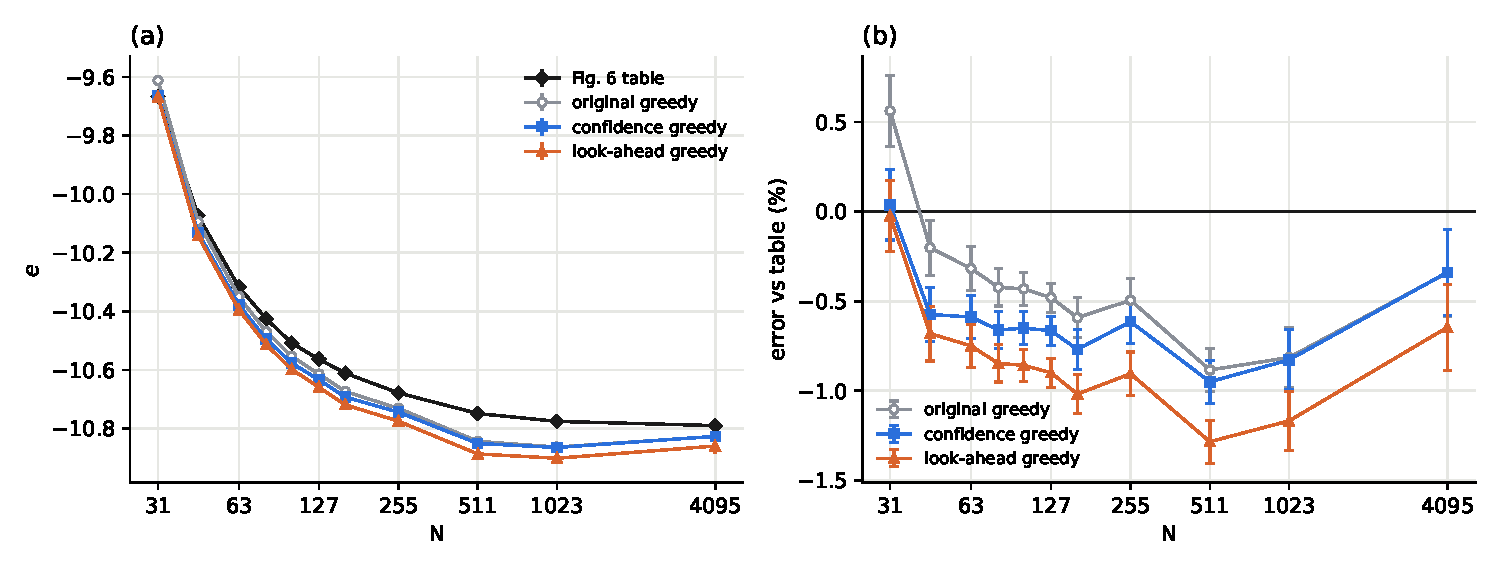
\includegraphics[width=\textwidth]{fig_energy.pdf}
  \caption{\textbf{Energies against the table:} (a) Average $e$ against $N$ for the table and the three greedy
  variants. (b) The same as an error against the table; error bars combine our standard error and the table's. Each
  greedy point averages fresh random instances: 20\,000 at small $N$, down to 60 at $N = 4095$. From our $N$ sweep
  and Stefan's Fig.~6 table.}
  \label{fig:energy}
\end{figure}

\begin{figure}[H]
  \centering
  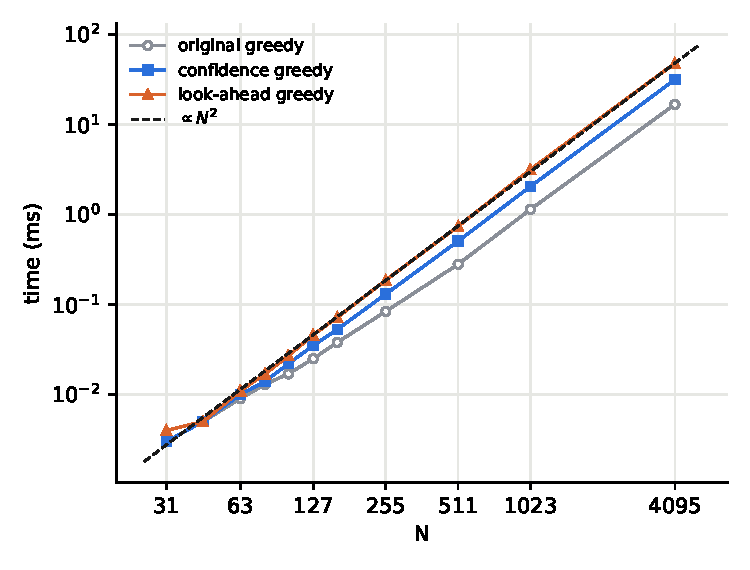
\includegraphics[width=0.6\textwidth]{fig_time.pdf}
  \caption{\textbf{Running time:} Time per instance on one Apple-silicon core, including the final descent. The
  dashed line is $\propto N^2$, anchored at the look-ahead greedy's $N = 4095$ point; all three variants follow it.
  From our $N$ sweep.}
  \label{fig:time}
\end{figure}

\begin{figure}[H]
  \centering
  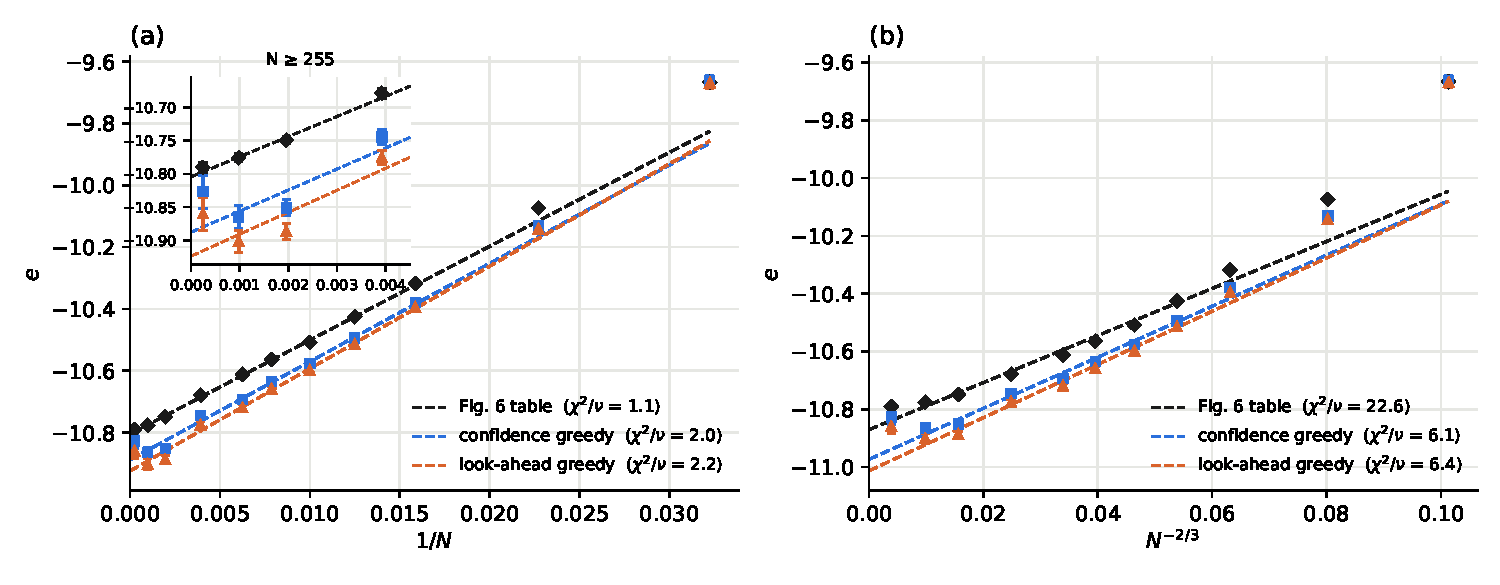
\includegraphics[width=\textwidth]{fig_extrap.pdf}
  \caption{\textbf{Extrapolation to large $N$:} (a) $e$ against $1/N$ with the fits $e_\infty + a/N$ (dashed); the
  inset zooms in on $N \ge 255$, where the greedy points at $N = 4095$ bend up away from their lines. (b) The same
  against $N^{-2/3}$, which fits the table much worse. Fits use $N \ge 63$. From our $N$ sweep and Stefan's table.}
  \label{fig:extrap}
\end{figure}

\begin{figure}[H]
  \centering
  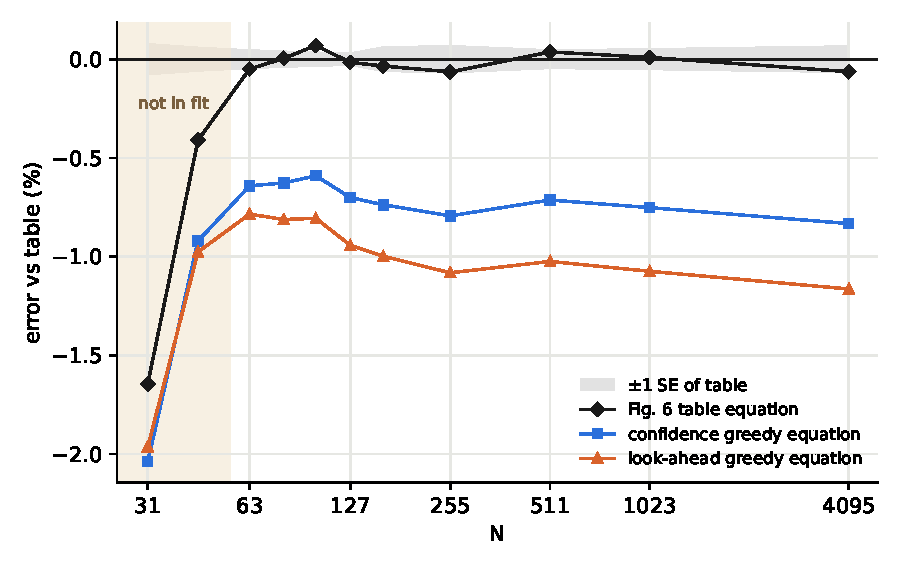
\includegraphics[width=0.75\textwidth]{fig_fitcheck.pdf}
  \caption{\textbf{How well each $1/N$ equation reproduces the table:} Each line is one fitted equation, evaluated at
  each $N$ and compared with the table value there; gray band: one standard error of the table. The table's own
  equation stays inside the band from $N = 63$ up. The greedy equations sit a nearly constant $0.6$--$1.2\%$ below the
  table: they describe the greedy energies, not the table. Shaded on the left: sizes left out of the fits.}
  \label{fig:fitcheck}
\end{figure}

\begin{figure}[H]
  \centering
  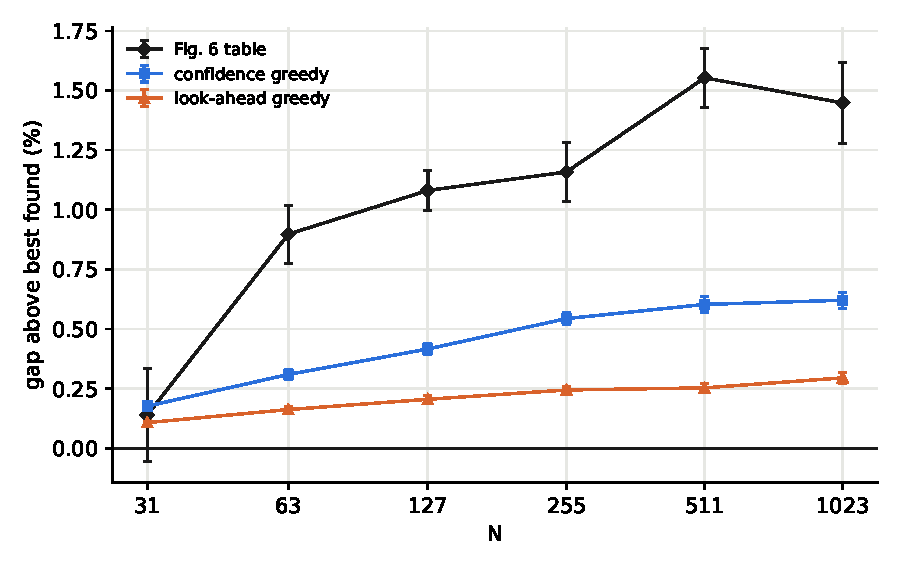
\includegraphics[width=0.75\textwidth]{fig_best.pdf}
  \caption{\textbf{Gap above the best energies found:} On 2000 instances at $N=31$, down to 60 at $N=1023$, we ran
  both greedy rules and a long tabu search (0.05\,s per instance at $N=31$, 10\,s at $N=1023$) on the same instances,
  and plot the average gap of each greedy rule above the tabu result. The table's gap is its error from
  Fig.~\ref{fig:energy} combined with the confidence greedy's gap. All three sit above the best found; the table is
  furthest above for $N \ge 63$ and agrees with it at $N = 31$. From the same-instance runs and Stefan's table.}
  \label{fig:best}
\end{figure}

\begin{figure}[H]
  \centering
  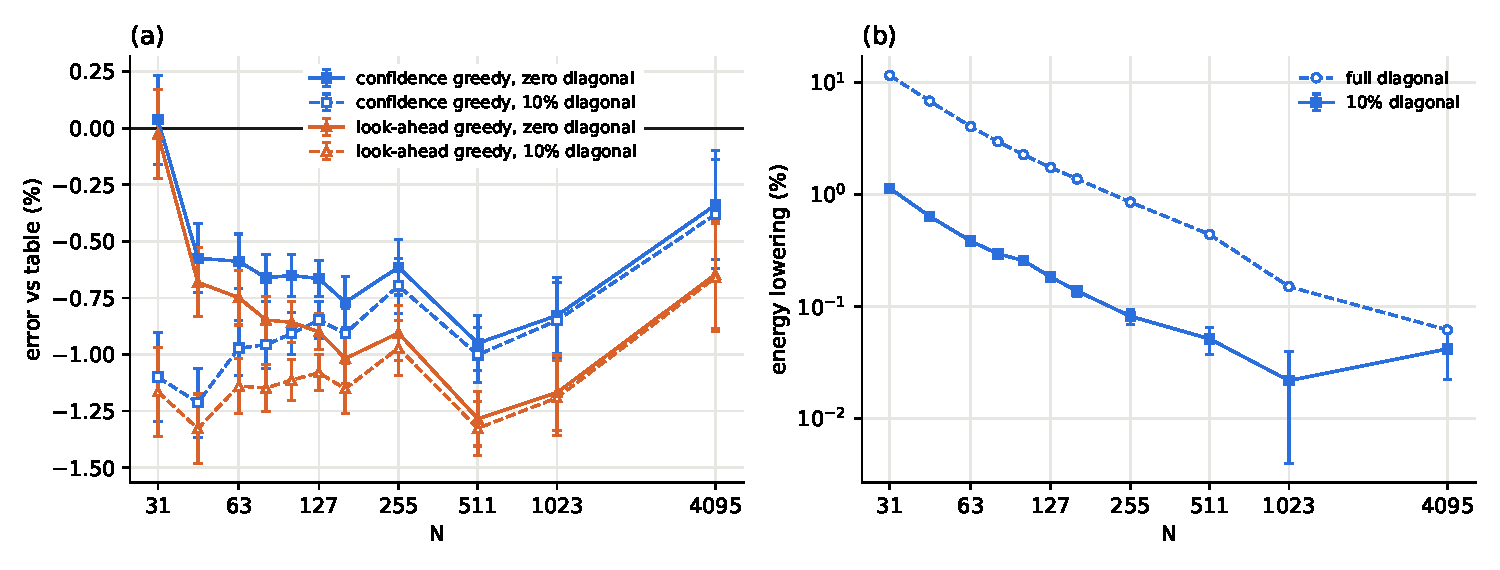
\includegraphics[width=\textwidth]{fig_diag.pdf}
  \caption{\textbf{What a nonzero diagonal would do:} (a) Error against the table with a zero diagonal (solid, as in
  Fig.~\ref{fig:energy}) and with a diagonal filled like the other entries (dashed): each diagonal entry nonzero with
  probability 0.1, then an integer from $[-100,100]$. The dashed points are the solid ones shifted by the paired
  change measured for each rule. (b) How much the diagonal lowers the greedy energy, for the
  10\% diagonal and for a fully filled one, as a percent of the table value. Both come from rerunning the confidence and
  look-ahead greedy on the same off-diagonal instances with and without the diagonal (20\,000 instances at small $N$,
  down to 60 at $N=4095$); the two rules give the same shift, so (b) shows the confidence greedy. The effect is large
  at small $N$ and falls off faster than $1/N$.}
  \label{fig:diag}
\end{figure}

\end{document}
